%
% 1.3
%
\section{Using Stata}%
	%
	%
	\label{sec:stata}%
	\index{Stata!Introduction}%
	%
	%
	
	\newthought{This course uses Stata} as its statistical software of choice. Stata is used by many social scientists working with quantitative data in areas such as economics and political science.%
	%
 	\footnote{For example, you will find Stata output in some of Nate Silver's work at the \emph{New York Times} on his `FiveThirtyEight' electoral blog; see, e.g., ``'\href{http://fivethirtyeight.blogs.nytimes.com/2012/03/12/polling-in-deep-south-has-posed-challenges/}{Polling in Deep South Has Posed Challenges},'' 12 March 2012.} %
	%
	Most statistical procedures used in these disciplines know some form of implementation in Stata, and the software is supported by a large user community that meets on the Statalist mailing-list and develops packages available through the Statistical Software Components (\SSC) server at Boston University. Overall, it is a solution that provides a good middle ground between a spreadsheet editor and a statistical programming environment. The next sections explain what that means and how Stata works.%

\newthought{The next sections} are based on commands and keyboard shortcuts that appear in Stata~12 for Mac~OS~X (Mac) and Windows (Win).%
		%
		\footnote{Compatible operating systems are listed at %
		\url{http://www.stata.com/products/compatible-operating-systems/}. %
		%
		We use the `Standard Edition' (\textsc{se}) of Stata that works on most current hardware.} %
		%
		Both systems run Stata almost similarly, with only a few notable differences:% 
		
	\begin{description}

		\item[\smallcaps{On Mac~OS~X}] %
		%
		The entire Stata application folder should be located in the \texttt{Applications} folder, and you should drag the Stata application icon to your Dock for quicker access. The \texttt{Cmd} (Command) key used in keyboard shortcuts is the `Apple' key located left and right of the spacebar.%

		\item[\smallcaps{On Windows}] %
		%
		The entire Stata application folder should be located in the \texttt{Program Files} folder, or whatever your version of Windows call it, and you should drag the Stata application icon to your Taskbar for quicker access. You might use either the 32-bit or 64-bit version of the software.%

	\end{description}

	The course should run fine on older versions of Stata, given very minor adjustments to the code. The course setup has been tested on Sciences Po workstations equipped with Stata~11, for which it automatically adjusts memory and circumvents admin restrictions to install packages.%
  \footnote{Known issues and fixes are documented at %
		\url{https://github.com/briatte/srqm/wiki/troubleshooting}}%
		
		
% 0.3.1
%
\subsection{Learning statistical software}%
	%
	%
	\newthought{You have probably never used Stata}, but you probably have some limited experience with number-crunching. For most users, this happens in a numerically inaccurate environment called a spreadsheet editor, in which you can freely delete or edit the data without letting others know. In that kind of environment, programming means writing functions into cells and then hoping for the cells to stay where they are, which they never do (Figure~\ref{fig:dilbert-spreadsheets}).%
		%
		\footnote{Read some horror stories compiled by the European Spreadsheet %
		Risks Interest Group (EuSpRIG): %
		\url{http://www.eusprig.org/horror-stories.htm}} %
		%
		A vast majority of jobs done in spreadsheet environments will not even explore that territory and will instead safely focus on showing unreadable `3D' pie charts with no meaningful third dimension.%
		%
		%

		\begin{figure}
			
\includegraphics{dilbert-excel}
		  \caption{\href{http://dilbert.com/strips/comic/2007-08-08/}{Dilbert on spreadsheets}, by Scott Adams.}%
		  \label{fig:dilbert-spreadsheets}%
		\end{figure}

	Your use of Stata in this course will remind you of a few things that you might have already learnt from using spreadsheet software. This will include using keyboard shortcuts a lot to move around the interface and to do things quicker, especially with respect to text manipulation. It will also include using filters and operators like \texttt{IF} or \texttt{MEAN} that you might know from functional programming in spreadsheets.%
		%
		%
	
	Statistical programming, on the other end, is probably new to you. Its general principle works more or less like writing music for a single musician: you have to compose a sequence of instructions that enables anyone to play your stuff. The current de facto standard in statistical programming is R, a free and open source software with excellent graphics support that lets you crunch numbers like a statistician would want you to: neatly, if at the cost of intuitiveness.%
		%
		\footnote{For example, in R, the number `2' is not just a number (i.e. a scalar), it is a vector of length 1 of numeric class.} %
		%
	 	R users know that its sheer complexity and subtle idiosyncracies create a steeper learning curve for new users, and that there is ``something not fully healthy''%
		\footnote{%
			\url{https://stat.ethz.ch/pipermail/r-help/2007-August/139047.html}} %
			about it. Still, if you ever plan to enhance your statistical programming skills, R and a few other languages will become your weapon of choice. Ivaylo and myself also teach an exploratory course in R if you want to get a feel of it.%
		\footnote{\url{http://f.briatte.org/teaching/ida/}}%
	%
	%

	\newthought{Stata is a compromise} between these two worlds that lets you work on a single spreadsheet of data through a set of predefined and user-contributed commands. It compares well to the competition: its emphasis on programming is more pronounced than what it is in SPSS, which is mostly used through point-and-click, and its language is more convenient than the one used by SAS, an expensive and historically dominant statistical software that remains the only solution capable of dealing with very large datasets. Stata is also less focused on a single approach to quantitative analysis than, say, Epi Info for epidemiology or gretl for econometrics.%
		%
		%
		
	Stata has its own limitations. Its graphics engine is not bad, but it is far from excellent: the graph syntax is tiresome, and it takes lines and lines of code to escape the default plots to produce better visualizations. Despite being rather open to user-contributed commands, Stata is a commercial product with a price tag and a closed proprietary format that requires conversion to import outside of Stata. Finally, and although that can be seen as a feature of the software, Stata can only work on a single dataset at a time, because it works like an accountant's book, one page after the other.%
		%
		%

% 0.3.2.
%
\index{Computers!Graphical User Interface (GUI)}%
\index{Computers!Command Line Interface (CLI)}%
\index{Stata!Command line interface}%
%
\subsection{Working from the command line} %
	%
	% graphical user interface
	% command line
	% example: sysuse lifeexp
	%
	Stata can be used either through its Graphical User Interface (GUI), like most of the software that you use, or through a Command Line Interface (CLI), which presents itself as a terminal where the user types instructions to produce certain results. The latter approach is the programmer's way of doing things: it is much more versatile and forces you to write up your operations in the form of a script, which Stata calls a `do-file'. This file is a plain text file containing Stata code that, like a music sheet, makes it possible to understand and reproduce your analysis of the original data.%
	
	We are going to explore Stata from the command line, which relies only on three windows: the Command line window, the Results window attached to it, and the do-files window. This minimal setup is shown below in Figure~\ref{fig:stata-ide}. We will not use any other element of the graphic user interface in this course, but feel free to explore Stata and learn about its other functionalities.%
	
	\begin{figure}
		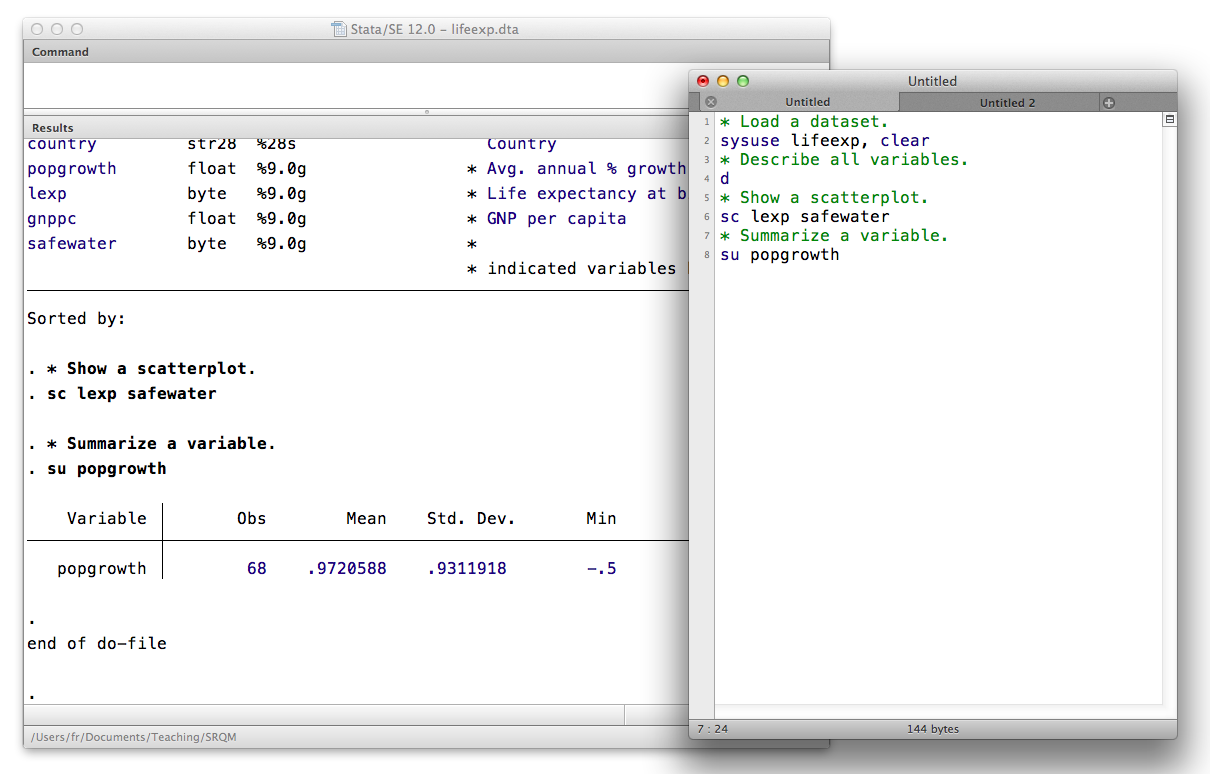
\includegraphics{stata-ide}%
		\caption{The Holy Trinity of Stata programming: the Command window (on top), the Results window (below it), and a do-file editor (in the background).}%
		\label{fig:stata-ide}%
	\end{figure}

%% -- command line

% The Stata GUI can be used occasionally for routine operations that need not appear in your do-files. Keyboard shortcuts also save some time, as with ‘File > Open…’ (Ctrl-O in Stata for Windows) or ‘File > Change Working Directory…’ (Cmmd-Shift-J in Stata for Macintosh; this document uses ‘Cmmd’ to designate the ‘’, a. k. a. ‘Command’, ‘Cmd’ or ‘Apple’ modifier key).

	The next sections explain how to run commands in Stata, and how to organize them into a do-file. A list of all commands used in the guide appear in the index, and a list of all commands used in the course appear on the course wiki.%
		\footnote{\url{https://github.com/briatte/srqm/wiki/synopsis}}%

		\begin{description}
			\item[\smallcaps{Running commands}]%
			\vspace{1em}%
			%
			In Stata, focus on the Command window by clicking into it or by pressing \texttt{Cmd-1} (Mac) or\texttt{Ctrl-1} (Win). Type the following command and press \texttt{Enter} to run the command, which means to execute its code:%
			
		\begin{docspec}%
			\label{lifeexp}%
			sysuse lifeexp, clear
		\end{docspec}
			
		If your command ran successfully, Stata will display its result:\\[1em]
			
			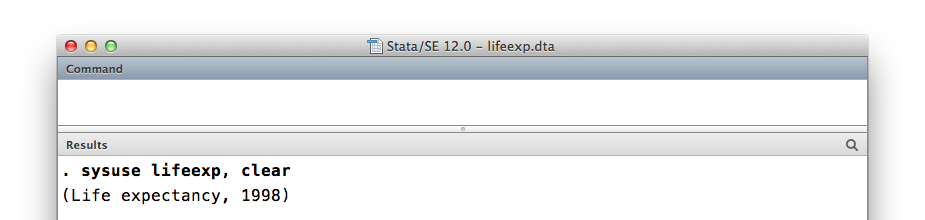
\includegraphics{stata-lifeexp-sysuse}\\[1em]

		Note that some commands produce `blank' output, which means that a command can be successfully entered and executed without printing any result. In this case, a simple \texttt{.} line dot will appear in the Results window, as to show that Stata encountered no problem while executing the command, and that it is ready to process another one.%
			%

			\item[\smallcaps{Fixing typos}] %
				\index{Stata!Syntax}%
			%
		Stata commands follow a strict syntax, and if you make a typo in a command, the software will return an error in red ink. In that case, you have to fix the issue by re-typing the command correctly. Try for example, to enter the following command:%
				%
				\marginnote{Examples with the \texttt{lifeexp} dataset %
					continued from p.~\pageref{lifeexp}.}%
			
			\begin{docspec}
				summarizze popgrowth
			\end{docspec}
			
			The mistake is rather obvious here: the \cmd[su]{summarize} command should take only one `z':\\[1em]%
			
			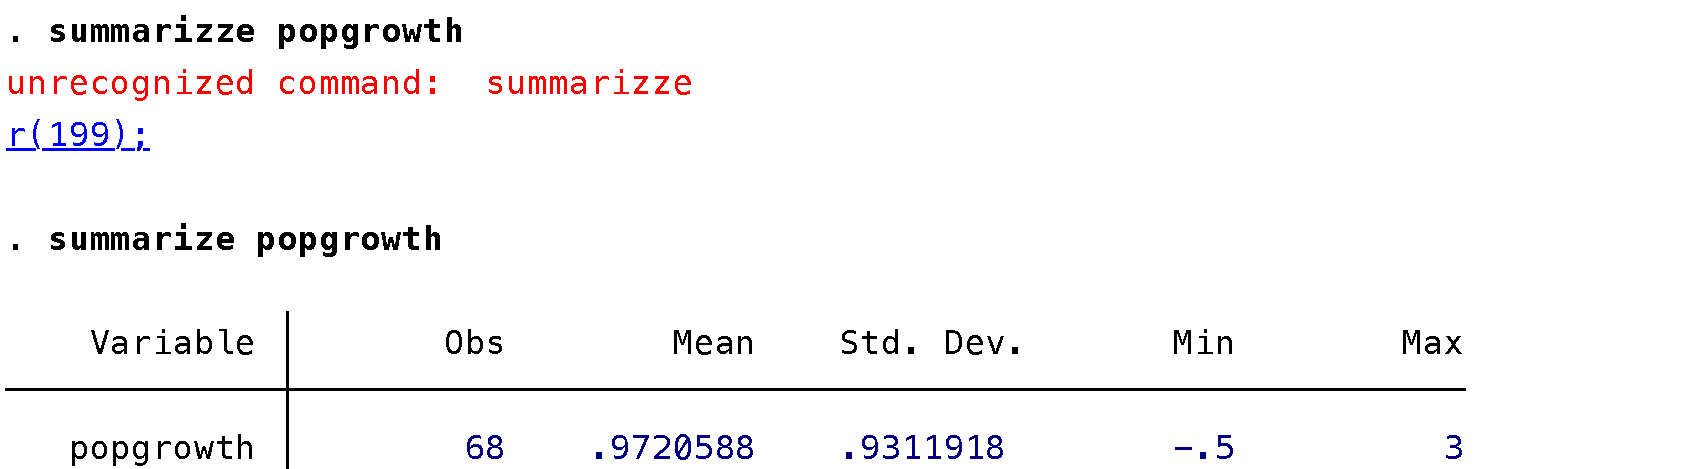
\includegraphics{lifeexp-sum-error-zz}\\[1em]
			
			If you need, as in this example, to correct a mispelled command, or to re-run a command that you have used earlier on, you should \textbf{press \texttt{PageUp} on your keyboard} to recall the previous command that you typed.%
			%
			\footnote{On laptop keyboards, \texttt{PageUp} is usually replaced by \texttt{Fn-UpArrow}. Past commands can also be examined in the Review window.} %
			%
			This allows you to fix your mistake by pulling the last command very quickly and correct only the typo, rather than having to type it again.%

			Here's another common mistake. Try the following in Stata:%
			
			\begin{docspec}
				Summarize popgrowth
				summarize POPGROWTH
			\end{docspec}

			In response to these commands, you will get more or less informative error messages. The issue here is that Stata commands are case-sensitive: the capitalized \texttt{Summarize} command is different from \texttt{summarize} command in lowercase. By that virtue, there is no variable called \texttt{POPGROWTH} in uppercase in the \texttt{lifeexp} dataset, but there is one called \texttt{popgrowth} in lowercase:\\[1em]%

			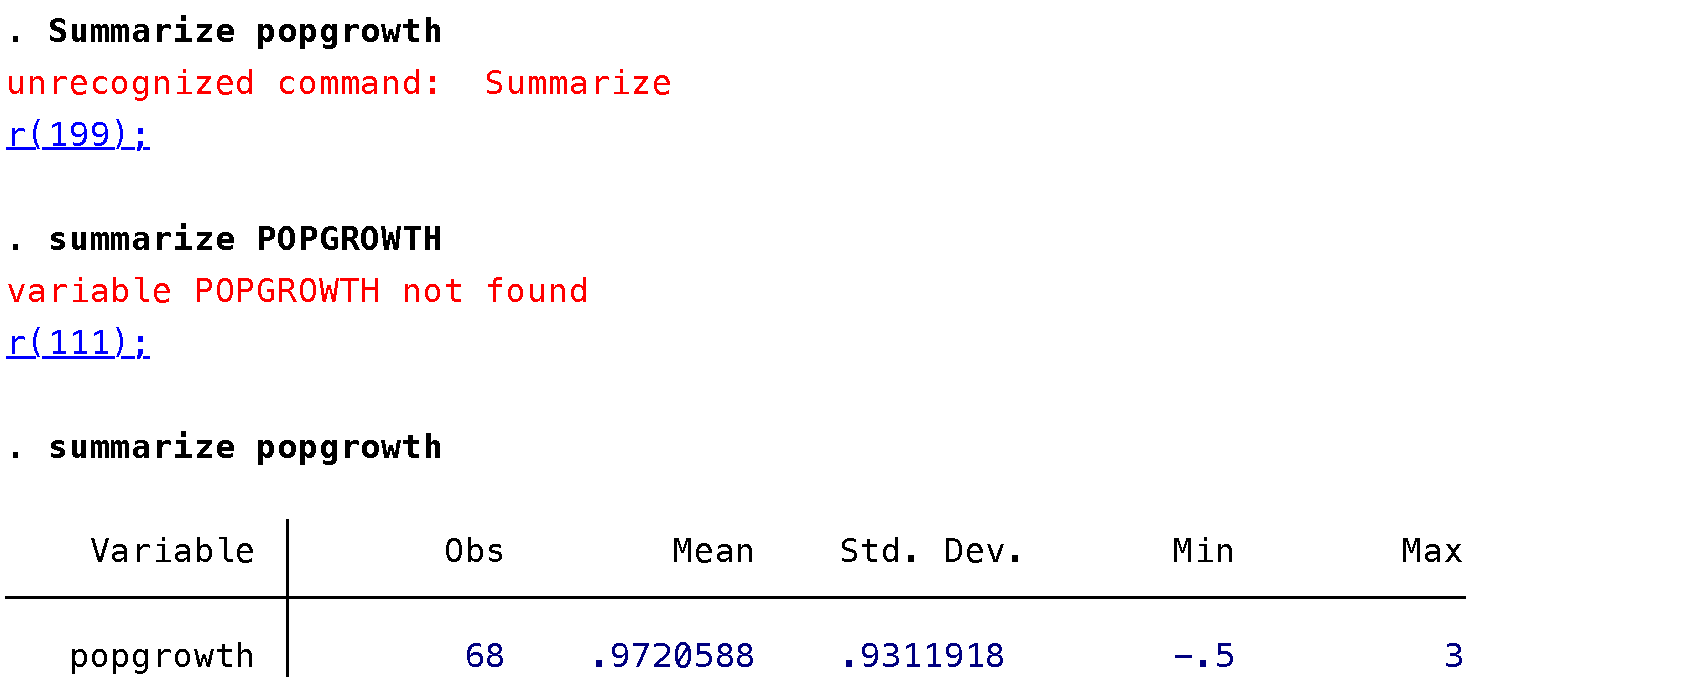
\includegraphics{lifeexp-sum-error-caps}\\[1em]
			
			Stata is usually operated in lowercase, although some variable names might show up in uppercase in some datasets. In order to keep things as straightforward as possible, avoid using uppercase yourself when naming variables.%
			
			%
			%
			\item[\smallcaps{Using help files}]%
				\index{Stata!Help files}
			%
			If you cannot find the right syntax or option for a command, turn to the technical documentation for precisions and examples of any given command. Use the \cmd[h]{help} command to access it in Stata, as in these examples:%
	
			\begin{docspec}
				* Help for the -summarize- command.\\
				help summarize\\[1em]
		
				* Help for the -lookfor- command.\\
				help lookfor
			\end{docspec}

			Stata help is also available online.%
				\footnote{\url{http://www.stata.com/help.cgi?help}} %
				
			\newthought{If you need further technical help} with Stata, refer to the course website for a selection of tutorials.%
				%
				\footnote{\url{http://f.briatte.org/teaching/quanti/}} %
				%
				A Web search with your question keywords might also work if someone has asked a similar question on Statalist or on StackOverflow.%
				%
				\footnote{\url{http://stackoverflow.com/}}%
				% 
				%

				\item[\smallcaps{Abbreviations}]%
					\index{Stata!Syntax}%
				%
				Most Stata commands can be abbreviated for quicker use. If you run the \texttt{help summarize} command, the help window will tell you that the \texttt{\underline{su}mmarize} command can be abbreviated to \texttt{su}. Type the following example in Stata to see how the language abbreviates:%
				%
				\marginnote{Examples with the \texttt{lifeexp} dataset %
					continued from p.~\pageref{lifeexp}.}%

		\begin{docspec}
			* With a command:\\%
			summarize popgrowth\\%
			su popgrowth\\[1em]%
			%
			* With help pages:\\%
			help summarize\\%
			h su%
		\end{docspec}

	Note that the bottom lines show you how to open help pages with the single letter \texttt{h}, which is handy when you are often brought to verify syntax and read examples from the documentation. This guide shows commands that can be abbreviated in both forms, as with \cmd[su]{summarize}, which is shown in the example:\\[1em]%

		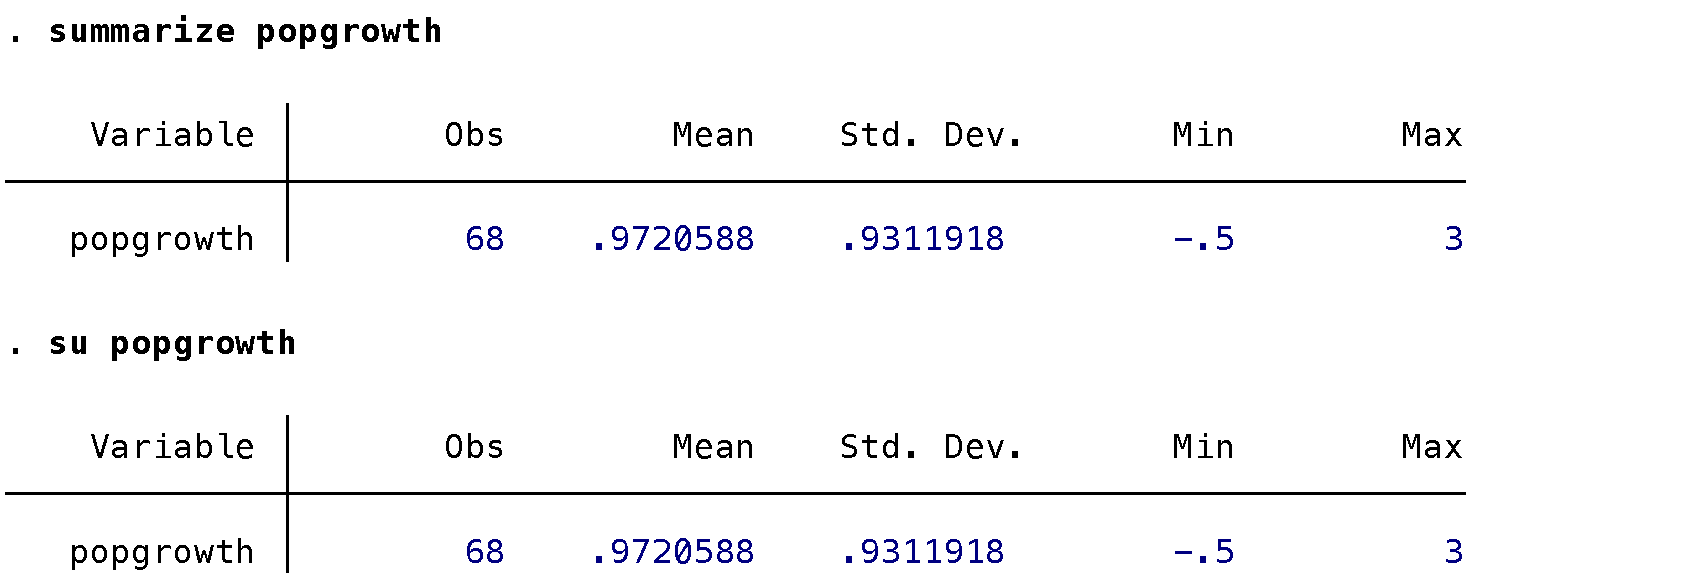
\includegraphics{lifeexp-summarize}\\[1em]

	Abbreviations exist for most commands and come in handy especially with commands such as \cmd[tab]{tabulate}, \cmd[d]{describe} or even \cmd[h]{help}. They also work for options like the \coab{d}{detail}{summarize} option for the \cmd[su]{summarize} command:\\[1em]%
	
		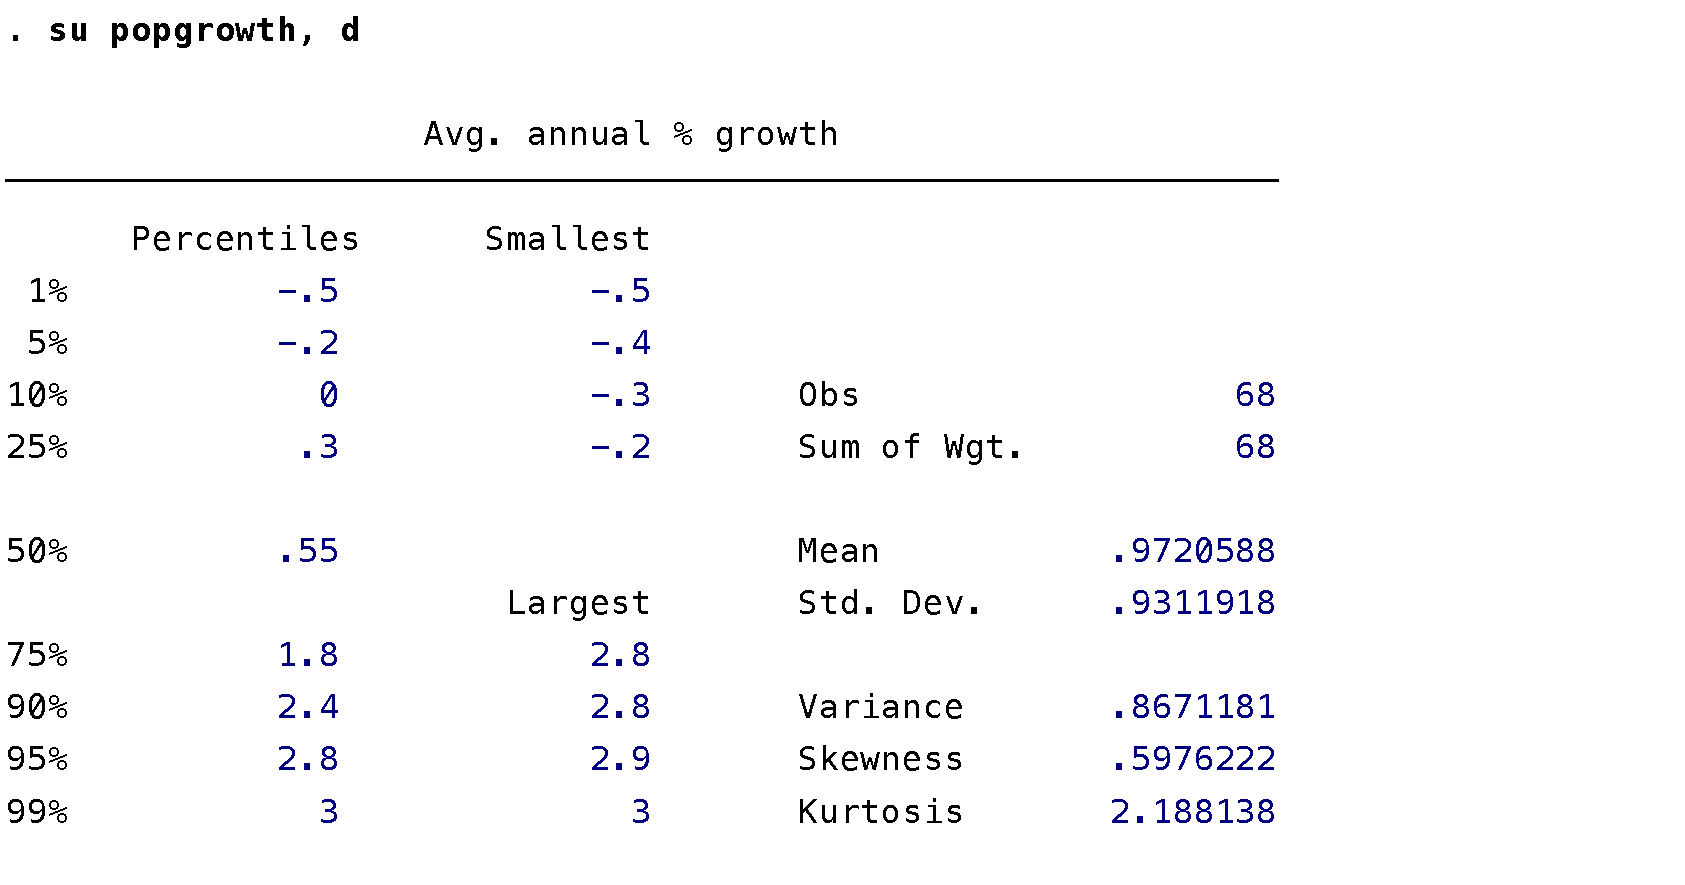
\includegraphics{lifeexp-summarize-d}\\[1em]

	%
	%
	\item[\smallcaps{Installing commands}]%
		\index{Stata!Packages (additional commands)}%
	%
	Stata can install additional commands written by users with programming skills. New commands can be installed by downloading packages from the \SSC server with the \cmd{ssc install} command, which is used at a few points in this guide to install some of these packages. You can install the \cmd{fre} command right away by typing the following command:%
		
	\begin{docspec}
		ssc install fre
	\end{docspec}
		
	Unless you are offline or already have installed the \cmd{fre} package, you should get a few result lines indicating where the package was installed on your hard drive:\\[1em]%
		
	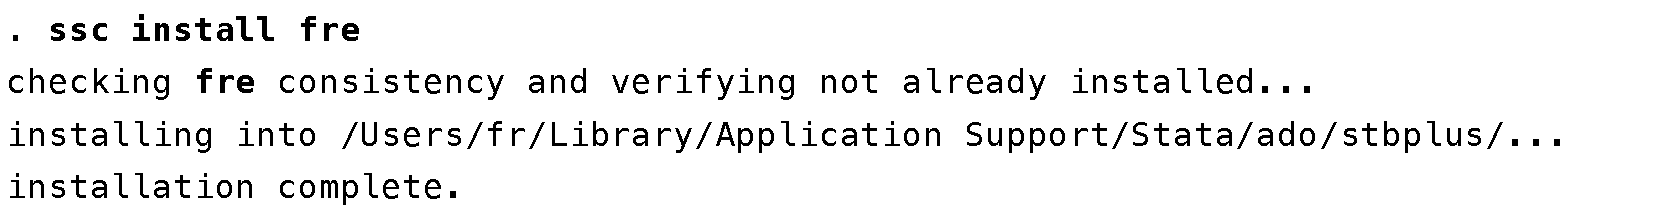
\includegraphics{ssc-install-fre}\\[1em]
		
	Other handy user-contributed commands have been installed as part of the course setup that you ran in the previous section.%
\end{description}

	%
	%
	\subsection{Working from a do-file}%
		\label{sec:do-files}%
		\index{Stata!Do-files}%
	%
	% command execution
	% comments
	% log
	%

	\index{Replication|seealso{Stata!Do-files}}%
	\newthought{When you run Stata commands} to explore a dataset, you are programming `on the fly', typing commands directly into the Stata command line to get quick results. But when you want to structure a complete analysis of your data, you need to record your commands to a script, which is a plain text file containing Stata code. An important part of your work in this course will therefore be to code your analysis into a script.%
	
	Coding your analysis is meant to provide yourself as well as others with the means to replicate your analysis. Maintaining a record of your operations—and commenting them inside as well as outside the code—will not only ensure that others can read and reproduce your work, but also that \emph{you} will be able to remember, in a few months or so, what you precisely ended up doing on your project.%
	
	Making your research fully replicable is not an option in this course: you are required to provide the code for your analysis. Replication also means that you should \hlred{\textbf{keep your original datasets unmodified}}: you will not need to save your modifications because you will instead save the instructions that allow any Stata user with the original data source to prepare it and analyze it as you have.%
	
	The logic of replicability (or reproducibility) outlined here 
	
	\newthought{Stata scripts} end with the \texttt{.do} extension and are called \textbf{do-files}.%
		 \footnote{Stata do-files will usually show as plain text in your Internet browser; if the browser adds a \texttt{.txt} extension to a do-file when downloading it, make sure that you rename the file to \texttt{.do} for Stata to recognize it as a do-file.} %
		%
		It will be one of your main missions throughout the course to learn how to structure and to write such a document. You will be given plenty of examples through a new course do-file every week, and the short vignette that follows will show you some essential aspects of working in Stata from a do-file.%
		%
		%
		
		\begin{marginfigure}
			
\includegraphics[width=.75\textwidth]{stata-do-icon}
			\caption{Stata~12 do-file icon.}
			\label{fig:stata-do}
		\end{marginfigure}

	\begin{description}
	\item[\smallcaps{Create an empty do-file}] Type \cmd{doedit} in the Command window to open a blank Stata do-file, which is your first piece of draft Stata code. Let's write a few lines into it:%

		\begin{docspec}
		  * François Briatte, first do-file\\[1em]%
			%
		  * Load UN data.\\%
			sysuse lifeexp, clear\\[1em]%
			%
			* Describe the data.\\%
			d\\[1em]%
			%
			* Summarize life expectancy\\%
			su lexp\\[1em]%
			%
			* Scatterplot.\\%
		  sc lexp safewater\\[1em]%
			%
			* ttyl\\
		\end{docspec}

		\emph{Step-by-step explanations:}
		
		\begin{enumerate}
			\index{Stata!Comments (code)}%
			\item First type in your name, preceded by an asterisk and a space. You will notice that the line will turn green, to indicate that it is a \textbf{comment}. Comments are for human readers of the code and are not evaluated by Stata, just passively printed to the Results window.%
			
			\item Now add the \cmd{sysuse} command that asks Stata to load a demo dataset in memory, removing any previous unsaved data. If you have run the previous examples, the same dataset will be loaded again.%
			
			\item Finally, add the \cmd[d]{describe} command to list the variables, the \cmd[su]{summarize} command to inspect the life expectancy variable, and the \cmd[sc]{scatter} command to produce a plot of the relationship between life expectancy and access to safe water.%

		\end{enumerate}

		Stata shows the code of your do-file in monospaced font with line numbers and colored syntax. The do-file editor should look like Figure~\ref{fig:hello-world-draft} on my system, which also highlights the currently selected line:%

		\begin{figure}%
			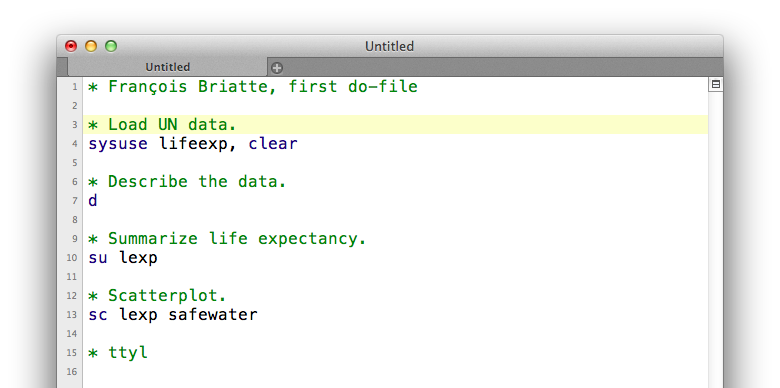
\includegraphics[width=\textwidth]{hello-world-draft}%
			\caption{A draft do-file using the \texttt{lifeexp} dataset.}%
			\label{fig:hello-world-draft}%
		\end{figure}

		\item[\smallcaps{Opening and saving do-files}] Once you are done copying and editing the demo code, save the do-file%
		%
		\footnote{Use \texttt{Cmd-S} (Mac) or \texttt{Ctrl-S} (Win) from your keyboard.} %
		%
		as \texttt{draft.do} in your \code folder, where you should keep all your do-files within the \SRQM folder.%
		
		Now close your first draft and return to the Stata Command window. If you have saved your draft as \texttt{draft.do} into the \code folder, as requested, then Stata will be able to open it with the following command:%

		\begin{docspec}
			doedit code/draft
		\end{docspec}
		
		The \cmd{doedit} command opens do-files from the current working directory, which should be the \SRQM folder for the duration of the course. You can open the course do-files by listing them in the \code folder, using a similar command to the one used previously with datasets:%
		
		
		 and then opening them with \cmd{doedit}.%
		
		
		\hlred{\textbf{{Note:} opening a do-file by double-clicking it is not recommended}, because Stata will quietly change the working directory to the location of the do-file.} The exact same problem exists with datasets. In both cases, you will have to set the working directory back to being the \SRQM folder.%

		Click anywhere on line 2 of your draft do-file and then press \texttt{Cmd-L} (Mac) or \texttt{Ctrl-L} (Win) to select it in full. Then, press \texttt{Shift+DownArrow} or \texttt{Shift+UpArrow} to select the line below or above it. Finally, press \texttt{Cmd-A} (Mac) or \texttt{Ctrl-A} (Win) to select all three lines.%
 
 		\item[\smallcaps{Running do-files}]

		To execute a do-file, press \texttt{Cmd-Shift-D} (Mac) or \texttt{Ctrl-D} (Win). The first line is a comment, as indicated by the asterisk at the beginning of the line, so executing it will not accomplish anything: Stata will just print it to the Results window.%
  
The second and third lines of your do-file will be printed to the Results window with their respective results. The \cmd{cd} command should print the path to your \SRQM folder, and the \cmd{di} command will print a `hello' message, as shown in Figure~\ref{fig:hello-world-result}.
  
\begin{figure}%
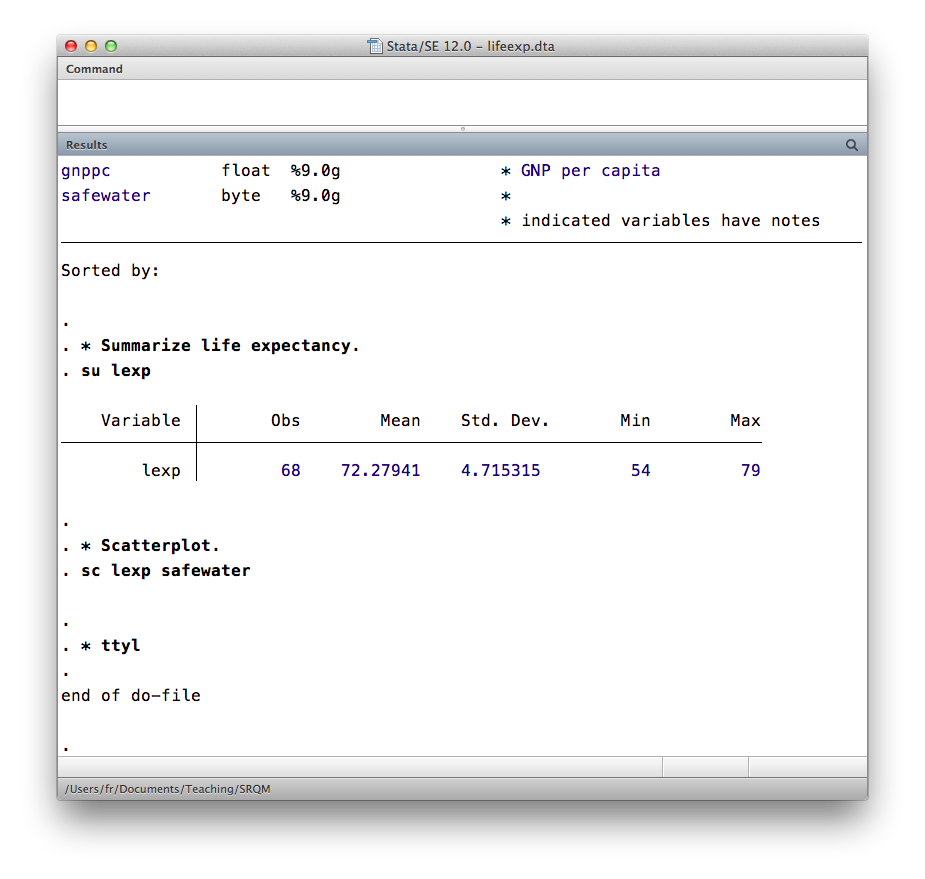
\includegraphics[width=\textwidth]{hello-world-result}
\caption{`Hello World' in Stata.}
\label{fig:hello-world-result}
\end{figure}

\hlred{\textbf{Important:} check your commands for typos and syntax errors.} If your code fails to execute, Stata will send some red ink to the Results window. Check the code against the correct syntax, looking for forgotten (or extra) letters or spaces.
  
\hlred{\textbf{Important:} be careful with copy-pasting to the Command window.} Copy-pasted commands that contain line breaks (\cmd{///}), for example, will not work properly. This point is covered again in the first course do-file.

% \item[Keyboard shortcuts]
  
You can switch between windows from the keyboard: use \texttt{Cmd-`} (Mac) or \texttt{Alt-Tab}. Have a look at the keyboard shortcuts in the `Window' command to learn similar tricks: for example, on Mac~OS~X, \texttt{Cmd-1} switches to the Command window.
  
%%% -- old : replication

The log is a text file that, once open with log using, will save every single command you enter in Stata as well as its results. Systematically logging your work is good prac-tice, even when you are just trying out a few things. Logs can be closed with the log close command followed by the name of your log if it has one:


Comments will also be saved to the log file, which is particularly useful when you have to read through your work again or share it with someone. In the example above, all comments, commands and results were saved to the log file.
% % %

Finally, open the first course do-file, which is your homework for the first week of class:

\begin{docspec}
doedit replication/week1
\end{docspec}

Follow the comments in this do-file to revise this section, learn a few more commands and briefly explore the course datasets.

%% -- old :: LOGS

Logs are useful to save every operation and result from a practice session. If you need someone else to replicate your work, however, you just need to share the commands you entered, along with the comments that you wrote to document your analysis. Files that contain commands and comments are called do-files.
Writing do-files is a crucial aspect of this course. Absent of a do-file, your work will be mostly incomprehensible, or at least impossible to reproduce, to others. Your do-file should include your comments, and it should run smoothly, without returning any er-rors. You will discover that these steps require a lot of work, so start to program early. To open a new do-file, use either the doedit command or the ‘File > New Do-file’ menu (keyboard shortcut: Ctrl-N on Windows, Cmmd-N on Macintosh).
You should take inspiration from the do-files produced for the course to write up your own do-file for your research project. All our do-files are available from the course web-site. This course requires only basic programming skills, as illustrated by the do-files that we run during our practice sessions. More sophisticated examples can be found online.
To execute (or ‘run’) a do-file, open it, select any number of lines, and press Ctrl-D in Stata for Windows or Cmmd-Shift-D in Stata for Macintosh. You can also use either the GUI icons on the top-right of the Do-file Editor window, or use the do or run com-mands. Use the Ctrl-L (Windows) or Cmmd-L (Macintosh) keyboard shortcuts to select the entire current line in order to run it.
Get some practice with do-files as soon as possible, since your coursework will include replicating one do-file a week. Replicating is nothing more than reading through the comments of a do-file, while running all its commands sequentially.

\end{description}
